% Usage: llmk optical.tex
% (if you are not using TeXLive < 2021, install llmk by yourself or execute, e.g.,
%   pdflatex -jobname=optical_1 optical.tex
% )

% Written in 2021 by Sho Iwamoto <webmaster@misho-web.com>
% To the extent possible under law, the author(s) have dedicated all copyright
% and related and neighboring rights to this software to the public domain
% worldwide. This software is distributed without any warranty.
% You should have received a copy of the CC0 Public Domain Dedication along with
% this software. If not, see http://creativecommons.org/publicdomain/zero/1.0/

%+++
% sequence=["optical1"]
%
% [programs.optical1]
% command="lualatex"
% opts=["-jobname=optical_1"]
%+++


\documentclass[12pt,a4paper]{article}
\usepackage{amsmath,amssymb,slashed,cancel}
\usepackage{graphicx,xcolor}
\usepackage[compat=1.1.0]{tikz-feynman}
\newcommand\w[1]{_{\mathrm{#1}}}
\usetikzlibrary{patterns}
\pgfrealjobname{optical}
\begin{document}
%===============================================================================
% Misho's dirty hack
%===============================================================================
\makeatletter
\pgfdeclaredecoration{sines}{initial}{
  \state{initial}[
    width=+0pt,
    next state=move,
    persistent precomputation={
      \def\tikzfeynman@cs@angle@step{30}
      \def\tikzfeynman@cs@current@angle{30}
      \pgfmathsetlengthmacro{\tikzfeynman@cs@points@per@step}{
        \pgfdecoratedinputsegmentlength
        / int(\pgfdecoratedinputsegmentlength
        / \pgfdecorationsegmentlength)
        / 360
        * \tikzfeynman@cs@angle@step}}]{}
  \state{move}[
    width=+\tikzfeynman@cs@points@per@step,
    next state=draw]{\pgfpathmoveto{\pgfpointorigin}}
  \state{draw}[
    width=+\tikzfeynman@cs@points@per@step,
    persistent postcomputation={
      \pgfmathparse{mod(\tikzfeynman@cs@current@angle+\tikzfeynman@cs@angle@step, 360)}
      \let\tikzfeynman@cs@current@angle=\pgfmathresult%
    },
  ]{
    \pgfmathparse{sin(\tikzfeynman@cs@current@angle) * \pgfmetadecorationsegmentamplitude / 2}
    \tikz@decoratepathfalse
    \pgfpathlineto{\pgfqpoint{0pt}{\pgfmathresult pt}}%
  }
  \state{final}{
    \ifdim\pgfdecoratedremainingdistance>0pt\relax\pgfpathlineto{\pgfpointdecoratedpathlast}\fi
  }
}
\makeatother
\tikzfeynmanset{/tikzfeynman/every boson@@/.style={
    /tikz/draw=none,
    /tikz/decoration={name=none},
    /tikz/postaction={
      /tikz/draw,
      /tikz/decoration={
        sines,
        meta-amplitude=1mm,
        segment length=8pt,
      },
      /tikz/decorate=true,
    }
}}

%===============================================================================
% Diagrams
%===============================================================================
% textwidth = 16 cm; 4cm x 2.46cm + 0.3cm margin
% dimension: 6x4cm
\def\tikzframe{
  \node (frame1) at (+2.0, -1.23) {};
  \node (frame2) at (+2.0, +1.23) {};
  \node (frame3) at (-2.0, -1.23) {};
  \node (frame4) at (-2.0, +1.23) {};
  \node (margin0) at (+2.3, -1.53) {};
  \node (margin2) at (+2.3, +1.53) {};
  \node (margin3) at (-2.3, -1.53) {};
  \node (margin4) at (-2.3, +1.53) {};
}



\beginpgfgraphicnamed{optical_1}%
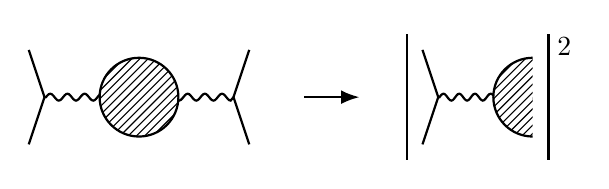
\begin{tikzpicture}[thick]
  \tikzframe
  \coordinate (c1)  at (-1.2, -0.5);
  \coordinate (c2)  at (+1.2, -0.5);
  \coordinate (mu1a) at (-1.4,  0.1);
  \coordinate (mu1b) at (-1.4, -1.1);
  \coordinate (mu2a) at (+1.4,  0.1);
  \coordinate (mu2b) at (+1.4, -1.1);

  \coordinate (xc1)  at ( 3.8, -0.5);
  \coordinate (xc2)  at (+6.2, -0.5);
  \coordinate (xmu1a) at ( 3.6,  0.1);
  \coordinate (xmu1b) at ( 3.6, -1.1);
  \coordinate (xmu2a) at ( 6.4,  0.1);
  \coordinate (xmu2b) at ( 6.4, -1.1);
  \begin{feynman}\diagram*{%
    (c1) -- [boson] (c2);
    (mu1a) -- (c1) -- (mu1b);
    (mu2a) -- (c2) -- (mu2b);
  };\end{feynman}%
  \filldraw[fill=white](0,-0.5) circle (0.5);
  \draw [-Latex](2.1,-0.5) -- (2.8,-0.5);
  \node [anchor=south] at (5.4, -0.1) {2};
  %  \filldraw[pattern=north east lines](0,-0.5) circle (0.5); [-0.5, 0] -- [0.5, -1]
  %  \filldraw[pattern=north east lines](5,-0.5) circle (0.5);
  % is the first touch but TikZ-pattern does not work quite well, so
   \begin{scope}
     \path[clip] (0,-0.5) circle (0.5);
     \foreach \t in {1,2,...,30}{
       \path[thin,draw] (2-0.052*\t, 0.052*\t) -- (-0.052*\t, -2+0.052*\t);
     }
   \end{scope}
  % right
  \draw (3.4, 0.3) -- (3.4, -1.3);
  \draw (5.2, 0.3) -- (5.2, -1.3);
  \begin{scope}
    \path[clip] (3.5, 0.3) rectangle (5, -1.3);
  \begin{feynman}\diagram*{%
    (xc1) -- [boson] (xc2);
    (xmu1a) -- (xc1) -- (xmu1b);
    (xmu2a) -- (xc2) -- (xmu2b);
  };\end{feynman}%
  \filldraw[fill=white](5,-0.5) circle (0.5);
  \path[clip] (5,-0.5) circle (0.5);
  \foreach \t in {1,2,...,30}{
    \path[thin,draw] (5+2-0.052*\t, 0.052*\t) -- (5-0.052*\t, -2+0.052*\t);
  }
  \end{scope}
\end{tikzpicture}

\endpgfgraphicnamed


\end{document}
